Для организации своей вычислительной инфраструктуры компании в настоящее время всё чаще выбирают решения, основанные на так называемых облачных платформах  \cite{fake-16}.
Такие решения имеют ряд достоинств, среди которых для данной работы наиболее важно следующее: загрузка аппаратного обеспечения может быть выше при организации инфраструктуры в облачное решение, чем при традиционной организации \cite{cloud-computing-concepts}.
Загрузка аппаратного обеспечения показывает какое количество аппаратных ресурсов используется относительно общего их количества \cite{fake-17}.
Чем выше загрузка, тем меньше аппаратных ресурсов работает вхолостую или простаивает.
Как холостая работа, так и простой ведут к прямым убыткам, в связи с чем более высокая загрузка обеспечивает финансовую выгоду \cite{fake-19}.

В облачных инфраструктурах повышение загрузки достигается с помощью разделения вычислительных ресурсов одного и того же сервера между несколькими задачами \cite{fake-20}.
В традиционной инфраструктуре такое разделение не применяется по причинам безопасности, а также из-за возможного захвата всех аппаратных ресурсов одной задачей и последующим простаиванием других \cite{fake-22}.
Таким образом, в традиционной архитектуре для выполнения того же объёма работы нужно больше аппаратных ресурсов, чем в облачной, как проиллюстрировано на рис.~\ref{load-utilization}.

\begin{figure}[hbtp]
    \centering
    \caption{Сравнение облачной и традиционной организации инфраструктуры}
    \label{load-utilization}
    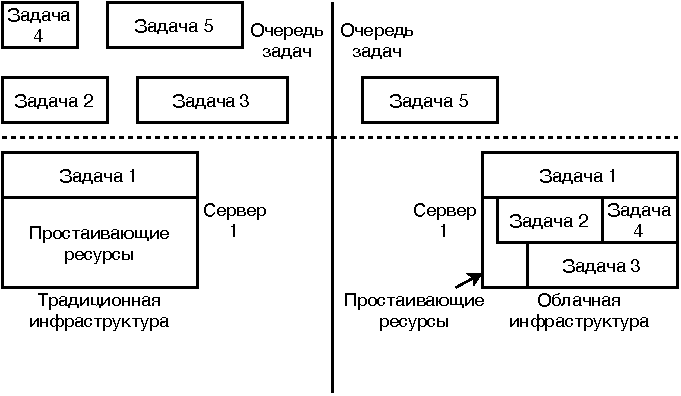
\includegraphics[width=13cm]{img/load-utilization.pdf}
\end{figure}

В облачных решениях захват всех аппаратных ресурсов невозможен вследствие ограниченного выделения ресурсов каждой из задач \cite{fake-23}.
В общем случае, это способы ограничения ресурсов делятся на два типа \cite{containers-and-vm-big-data}:
\begin{itemize}
    \item решения на базе виртуальных машин;
    \item решения на базе контейнеров.
\end{itemize}

В обоих подходах количество ресурсов, доступных задаче, управляются с помощью:
\begin{itemize}
    \item количества таких виртуальных машин или контейнеров;
    
    Этот способ называется ''масштабирование''.
    \item количества ресурсов, доступных одной виртуальной машине или одному контейнеру.
\end{itemize}

Масштабирование в настоящее время применяется чаще \cite{fake-24} по ряду причин, среди которых:
\begin{itemize}
    \item возможность выделения на одно приложение (задачу) несколько серверов за счёт запуска виртуальных машин или контейнеров на каждом из них \cite{fake-28}.
    \item Более высокая загрузка оборудования, так как в случае отсутствия нагрузки на приложение, будет простаивать только то количество аппаратных ресурсов, которое выделено одной виртуальной машине или контейнеру приложения, другие ресурсы при этом будут высвобождены \cite{fake-25}.
    В случае масштабирования есть возможность выделить одной виртуальной машине или контейнеру минимально необходимое количество ресурсов для обработки минимальной нагрузки на приложение, в то время как при выделении ресурсов, достаточных для обработки пиковой нагрузки, будет наблюдаться простой в обычном режиме работы \cite{fake-26}. 
\end{itemize}

Таким образом, существует задача масштабирования приложений.
Для решения этой задачи существуют технологии, имеющие общее название ''автомасштабирование'' \cite{portable-autoscaler-for-managing-multi-cloud-elasticity}.
При помощи таких технологий осуществляется автоматическое масштабирование в зависимости от текущей нагрузки на приложение или других факторов.

Во многие платформы облачных вычислений сервисы автомасштабирования уже встроены \cite{fake-32}, однако существуют сервисы автомасштабирования, являющиеся внешними по отношению к платформе.
Причины появления таких сервисов могут быть разными:
\begin{itemize}
    \item отсутствие решений автомасштабирования в используемой облачной платформе \cite{fake-27};
    \item более эффективная реализация автомасштабирования у внешнего решения, чем у встроенного.
    Это может быть обусловлено как спецификой конкретного приложения, на которое платформа не рассчитана, так и недостаточной эффективностью встроенного решения \cite{fake-29}.
\end{itemize}
На практике зачастую внешние сервисы автомасштабирования спроектированы и разработаны под одну конкретную платформу облачных вычислений и не могут взаимодействовать с другими \cite{fake-30}.

В случае, если система состоит из нескольких разных облачных платформ или в системе осуществляется миграция с одной облачной платформы на другую, появляется необходимость в существенной доработке сервиса автомасштабирования, если он был спроектирован лишь под одну платформу \cite{fake-31}.
Далее в этой главе будет представлен обзор научных работ, статей и патентов, посвящённых решению описанной проблемы.
